% !TeX root = ../../../geos_mpm_manual.tex
\section{Particle types and interpolation/update options}
\label{sec:particle-types-and-mapping}
\index{particle types}
\index{particle mapping}
\index{CPDI}
\index{B-spline}
\index{PIC}
\index{FLIP}
\index{XPIC}
\index{FMPM}

This section documents the interpolation and particle update choices used by the MPM solver.  The user-facing particle-type controls are generated by ParticleFileWriter and are summarized with the other material, group, and particle-type controls in Section~\ref{sec:pfw-materials}; this section focuses on the internal numerical operators.  The reviewed code exposes the particle-type enumeration
\begin{equation}
  \texttt{SinglePoint},\quad
  \texttt{SinglePointBSpline},\quad
  \texttt{CPDI},\quad
  \texttt{CPTI},\quad
  \texttt{CPDI2},
\end{equation}
and the velocity/state update enumeration
\begin{equation}
  \texttt{FLIP},\quad \texttt{PIC},\quad \texttt{XPIC},\quad \texttt{FMPM}.
\end{equation}
The implemented particle setup paths in the reviewed source are \texttt{SinglePoint}, \texttt{SinglePointBSpline}, and \texttt{CPDI}.  The \texttt{CPTI} and \texttt{CPDI2} identifiers are reserved for future development; attempting to generate those particle types in the reviewed particle setup path raises a not-implemented error.  The same particle-to-grid and grid-to-particle mapping data are reused by the force, kinematic, contact, boundary, and diagnostic steps described in Sections~\ref{sec:solver-steps} and~\ref{sec:bc-internals}.

\subsection{Mapping notation and effective support}
\label{subsec:mapping-notation}
\index{particle mapping!notation}

Let $p$ denote a material point, $I$ a background-grid node, $m_p$ the particle mass, $V_p$ the particle volume, $\boldsymbol{x}_p$ the particle position, $\boldsymbol{v}_p$ the particle velocity, and $\boldsymbol{\sigma}_p$ the Cauchy stress.  The solver stores, for each active particle, a sparse set of mapped nodes together with shape values $N_{Ip}$ and gradients $\boldsymbol{\nabla}N_{Ip}$.  These quantities define the standard MPM projections
\begin{align}
  m_I &= \sum_p m_p N_{Ip},
  &
  \boldsymbol{p}_I &= \sum_p m_p \boldsymbol{v}_p N_{Ip},
  &
  \boldsymbol{v}_I &= \frac{\boldsymbol{p}_I}{m_I},
  \label{eq:mpm-p2g-mass-momentum}\\
  \boldsymbol{f}^{\mathrm{int}}_I
    &= -\sum_p V_p\,\boldsymbol{\sigma}_p\boldsymbol{\nabla}N_{Ip},
  &
  \boldsymbol{L}_p
    &= \sum_I \boldsymbol{v}_I\otimes \boldsymbol{\nabla}N_{Ip},
  \label{eq:mpm-p2g-force-gradient}
\end{align}
with additional material-field or group labels used when contact and boundary branches need split nodal states.  Equations~\eqref{eq:mpm-p2g-mass-momentum} and~\eqref{eq:mpm-p2g-force-gradient} are the common PIC/FLIP MPM transfer operators introduced for solid mechanics by Sulsky, Chen, and Schreyer and later generalized through GIMP, CPDI, and related domain methods \cite{sulsky1994history,sulsky1995solid,bardenhagen2004gimp,sadeghirad2011cpdi}.

The implementation distinguishes a raw geometric support from an effective support.  For \texttt{SinglePoint}, the raw map has the eight trilinear nodes of the cell containing the particle.  For \texttt{SinglePointBSpline}, the raw map has the $4^3=64$ tensor-product cubic B-spline control nodes surrounding the particle.  For \texttt{CPDI}, each of the eight particle-domain corners contributes eight trilinear nodes, again giving as many as 64 raw entries.  A coalescing pass combines repeated grid nodes, sums their contributions, removes zero entries, and provides the effective map used by most particle-to-grid and grid-to-particle kernels.  This detail matters because CPDI corners may share grid nodes after distortion or near grid boundaries, and because B-spline support is broader than linear MPM support even though it is still driven by a single particle center.

\subsection{Single-point particles with trilinear mapping}
\label{subsec:single-point-linear}
\index{SinglePoint}
\index{particle mapping!single point}

The \texttt{SinglePoint} type is the classical point-quadrature MPM discretization.  The particle characteristic function is a Dirac measure located at $\boldsymbol{x}_p$, and the background basis is the trilinear finite-element basis on the cell containing the particle.  If $\boldsymbol{h}=(h_x,h_y,h_z)$ is the local cell spacing and
\begin{equation}
  \boldsymbol{s}=(s_x,s_y,s_z),
  \qquad
  s_d=\frac{x_{p,d}-x_{0,d}}{h_d}\in[0,1],
  \label{eq:single-point-local-coord}
\end{equation}
are the local coordinates measured from the lower cell corner, then the one-dimensional linear weights are
\begin{equation}
  \ell_0(s)=1-s,
  \qquad
  \ell_1(s)=s,
  \qquad
  \frac{d\ell_0}{dx}=-\frac{1}{h},
  \qquad
  \frac{d\ell_1}{dx}=\frac{1}{h}.
  \label{eq:linear-mpm-weights}
\end{equation}
For a node with local index $\boldsymbol{a}=(a_x,a_y,a_z)$, $a_d\in\{0,1\}$,
\begin{align}
  N_{\boldsymbol{a}p}
    &= \ell_{a_x}(s_x)\ell_{a_y}(s_y)\ell_{a_z}(s_z),
  \label{eq:linear-mpm-shape}\\
  \frac{\partial N_{\boldsymbol{a}p}}{\partial x}
    &= \frac{d\ell_{a_x}}{dx}(s_x)\ell_{a_y}(s_y)\ell_{a_z}(s_z),
  \label{eq:linear-mpm-grad-x}
\end{align}
with cyclic permutations for $y$ and $z$.  The weights satisfy partition of unity and reproduce linear fields inside a cell, but the gradient is discontinuous at cell boundaries.  Consequently, standard point MPM is susceptible to cell-crossing noise and quadrature error when particles move from one background cell to another.  These errors motivated the generalized interpolation material point method, smoother basis studies, CPDI, and related projection improvements \cite{bardenhagen2004gimp,steffen2008quadrature,steffen2008choices,wallstedt2007projection}.

In the reviewed implementation the \texttt{SinglePoint} generator stores a volume and visualization domain vectors, but the interpolation itself uses only the particle center.  The stored domain vectors allow the particle file and plotting tools to display a finite volume, while the map used by Equations~\eqref{eq:mpm-p2g-mass-momentum}--\eqref{eq:mpm-p2g-force-gradient} remains the eight-node point map in Equation~\eqref{eq:linear-mpm-shape}.

\subsection{Single-point particles with cubic B-spline mapping}
\label{subsec:single-point-bspline}
\index{SinglePointBSpline}
\index{B-spline!cubic}
\index{particle mapping!B-spline}

The \texttt{SinglePointBSpline} type keeps the particle as a point quadrature rule but replaces the trilinear cell basis by a tensor-product cubic cardinal B-spline basis.  The support is four nodes in each direction, giving $64$ grid nodes in three dimensions.  Let
\begin{equation}
  u_d = \frac{x_{p,d}-x^{\min}_d}{h_d},
  \qquad
  i_d=\lfloor u_d\rfloor,
  \qquad
  s_d=u_d-i_d\in[0,1),
\end{equation}
and let the first supported node in direction $d$ be $i_d-1$.  For one dimension, the four nonzero cubic B-spline weights used by the solver are
\begin{align}
  b_0(s) &= \frac{(1-s)^3}{6},
  &
  b_1(s) &= \frac{3s^3-6s^2+4}{6},
  \label{eq:bspline-cubic-weights-a}\\
  b_2(s) &= \frac{-3s^3+3s^2+3s+1}{6},
  &
  b_3(s) &= \frac{s^3}{6}.
  \label{eq:bspline-cubic-weights-b}
\end{align}
Their derivatives with respect to physical position are
\begin{align}
  \frac{db_0}{dx} &= -\frac{(1-s)^2}{2h},
  &
  \frac{db_1}{dx} &= \frac{1.5s^2-2s}{h},
  \label{eq:bspline-cubic-grads-a}\\
  \frac{db_2}{dx} &= \frac{-1.5s^2+s+0.5}{h},
  &
  \frac{db_3}{dx} &= \frac{s^2}{2h}.
  \label{eq:bspline-cubic-grads-b}
\end{align}
The three-dimensional basis is the tensor product
\begin{equation}
  N_{\boldsymbol{a}p}=b_{a_x}(s_x)b_{a_y}(s_y)b_{a_z}(s_z),
  \qquad
  a_d\in\{0,1,2,3\},
  \label{eq:bspline-tensor-product}
\end{equation}
and the gradient is obtained by differentiating the one-dimensional factor in the selected coordinate direction.  The code applies a deterministic closure correction to the final supported node so that the sum of the stored shape values is exactly one and the sum of the stored gradients is exactly zero to roundoff.

The motivation for this option is the same as in smoother-basis MPM studies: broader, smoother basis functions reduce force and velocity projection jumps when particles cross grid-cell boundaries.  Steffen et al. analyzed implementation choices and quadrature errors in MPM, and later B-spline MPM work showed that B-spline bases can reduce cell-crossing artifacts and improve continuity of grid fields \cite{steffen2008quadrature,steffen2008choices,gan2018bspline}.  The GEOS option should be interpreted as a single-point B-spline quadrature choice, not as a finite particle-domain method: the particle center controls the interpolation, while the stored particle domain vectors are retained for volume accounting and output.

\begin{figure}[tbp]
  \centering
  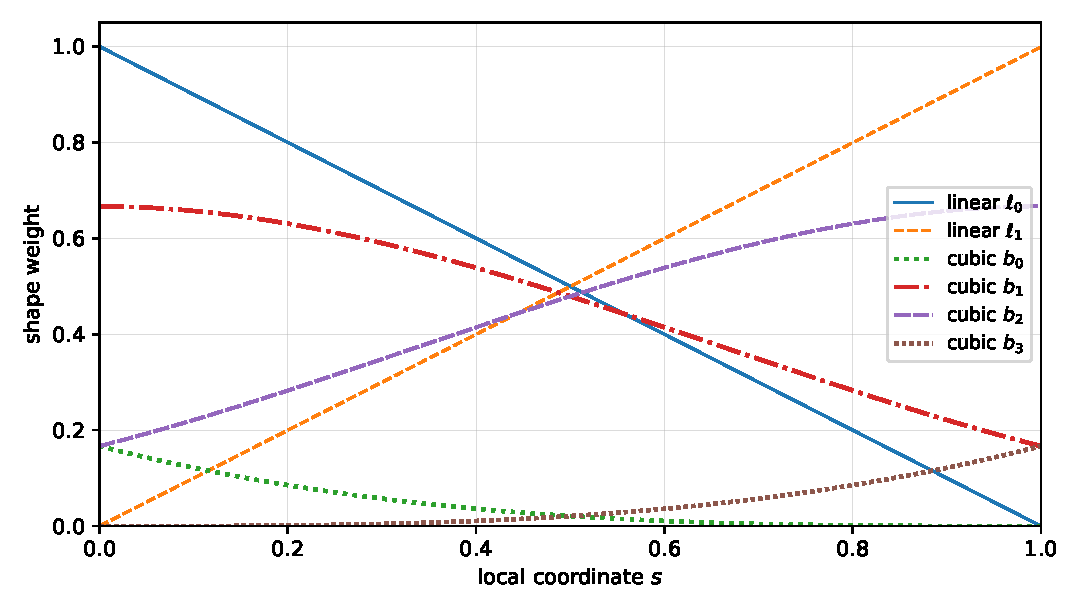
\includegraphics[width=0.92\linewidth]{figures/particle_shape_functions.pdf}
  \caption{One-dimensional shape functions used to build the tensor-product maps.  The linear MPM map has two active weights on the host cell, whereas the cubic B-spline map has four active weights with $C^2$ continuity across cell interfaces.  The three-dimensional maps are tensor products of these one-dimensional functions.}
  \label{fig:particle-shape-functions}
\end{figure}

\begin{lstlisting}[caption={Single-point cubic B-spline map construction.},basicstyle=\ttfamily\small]
for each active particle p:
  for d in x,y,z:
    u = (x_p[d] - grid_min[d]) / h[d]
    cell = floor(u)
    s = u - cell
    base[d] = cell - 1
    compute b[0:4](s) and dbdx[0:4](s)
  for a,b,c in 0..3:
    I = node(base[x]+a, base[y]+b, base[z]+c)
    N_Ip = bx[a] * by[b] * bz[c]
    gradN_Ip = (dbx[a]*by[b]*bz[c],
                 bx[a]*dby[b]*bz[c],
                 bx[a]*by[b]*dbz[c])
  adjust last entry so sum(N)=1 and sum(gradN)=0
\end{lstlisting}

\subsection{CPDI with trilinear background shape functions}
\label{subsec:cpdi-linear}
\index{CPDI}
\index{particle domain}
\index{particle mapping!CPDI}

The \texttt{CPDI} type implements convected particle domain interpolation for a parallelepiped particle domain.  CPDI replaces point evaluation of the grid basis by a particle-domain average, thereby reducing cell-crossing noise and improving behavior under large deformation.  This follows the convected particle domain interpolation method of Sadeghirad, Brannon, and Burghardt \cite{sadeghirad2011cpdi}.  In GEOS, the particle carries a center $\boldsymbol{x}_p$ and three half-edge vectors $\boldsymbol{r}_1$, $\boldsymbol{r}_2$, and $\boldsymbol{r}_3$.  The current domain is
\begin{equation}
  \Omega_p = \left\{
  \boldsymbol{x}_p+\xi_1\boldsymbol{r}_1+
  \xi_2\boldsymbol{r}_2+
  \xi_3\boldsymbol{r}_3
  \;:\;
  -1\le \xi_1,\xi_2,\xi_3\le 1
  \right\},
  \label{eq:cpdi-domain}
\end{equation}
with volume
\begin{equation}
  V_p = 8\,\boldsymbol{r}_1\cdot(\boldsymbol{r}_2\times\boldsymbol{r}_3).
  \label{eq:cpdi-volume}
\end{equation}
For the eight corners $c$, define signs $s^c_i\in\{-1,1\}$ and corner positions
\begin{equation}
  \boldsymbol{x}^c_p = \boldsymbol{x}_p
   +s^c_1\boldsymbol{r}_1+s^c_2\boldsymbol{r}_2+s^c_3\boldsymbol{r}_3.
  \label{eq:cpdi-corners}
\end{equation}
The GEOS map evaluates the background trilinear shape functions at each corner and assigns one-eighth of the corner contribution to the particle map,
\begin{equation}
  \overline{N}_{Ip}
  \approx \frac{1}{8}\sum_{c=1}^{8} N_I(\boldsymbol{x}^c_p).
  \label{eq:cpdi-shape-average}
\end{equation}
For gradients, let
\begin{equation}
  \boldsymbol{A}=\boldsymbol{r}_2\times\boldsymbol{r}_3,
  \qquad
  \boldsymbol{B}=\boldsymbol{r}_3\times\boldsymbol{r}_1,
  \qquad
  \boldsymbol{C}=\boldsymbol{r}_1\times\boldsymbol{r}_2.
  \label{eq:cpdi-area-vectors}
\end{equation}
The corner gradient coefficient used internally is
\begin{equation}
  \boldsymbol{\alpha}^c_p
  =\frac{s^c_1\boldsymbol{A}+s^c_2\boldsymbol{B}+s^c_3\boldsymbol{C}}{V_p},
  \label{eq:cpdi-alpha}
\end{equation}
and the effective gradient is assembled as
\begin{equation}
  \boldsymbol{\nabla}\overline{N}_{Ip}
  \approx \sum_{c=1}^{8} N_I(\boldsymbol{x}^c_p)\,\boldsymbol{\alpha}^c_p.
  \label{eq:cpdi-gradient-average}
\end{equation}
Equations~\eqref{eq:cpdi-shape-average}--\eqref{eq:cpdi-gradient-average} are stored initially as corner/node raw entries and then coalesced by grid node.  A closure adjustment enforces the corner partition of unity and gradient consistency before the raw entries are merged.

\begin{lstlisting}[caption={CPDI map construction for a parallelepiped particle domain.},basicstyle=\ttfamily\small]
for each active CPDI particle p:
  A = r2 x r3; B = r3 x r1; C = r1 x r2
  V = 8 * dot(r1,A)
  for each corner sign sc in {-1,1}^3:
    x_c = x_p + sc[0]*r1 + sc[1]*r2 + sc[2]*r3
    alpha_c = (sc[0]*A + sc[1]*B + sc[2]*C) / V
    evaluate eight trilinear grid weights N_I(x_c)
    for each corner node I:
      raw_N_Ip     += (1/8) * N_I(x_c)
      raw_grad_Ip  += alpha_c * N_I(x_c)
  coalesce duplicate nodes and enforce consistency corrections
\end{lstlisting}

CPDI remains a background-grid method: nodal equations are still solved on the rectilinear grid, but the particle basis carries an evolving domain.  The particle domain vectors are updated by the deformation history, and the volume used in the stress divergence reflects the convected domain.  This is especially important for large tensile strains and rotations, where point MPM may develop severe quadrature error or numerical fracture.  The domain-averaged CPDI map trades a larger stencil for smoother transfer and a more physically meaningful particle support \cite{sadeghirad2011cpdi,homel2016domaindef}.

\subsection{CPDI domain scaling}
\label{subsec:cpdi-domain-scaling}
\index{CPDI!domain scaling}
\index{domain scaling}
\index{VP-Hencky domain scaling}
\index{numerical fracture}

The optional CPDI domain-scaling step regularizes only the particle domain used for CPDI integration and mapping.  It does not replace the constitutive deformation gradient.  Before each map, the solver first reconstructs the unscaled current half-edge vectors from the physical deformation gradient and the reference domain,
\begin{equation}
  \boldsymbol{r}_{a}=\mathbf{F}\boldsymbol{r}^{0}_{a},
  \qquad a=1,\ldots,d,
  \label{eq:cpdi-raw-domain-from-f}
\end{equation}
where $d=2$ for plane strain and $d=3$ otherwise.  The input \texttt{cpdiDomainScalingType} selects either the compatibility method \texttt{homel}, which is the default, or the fixed-measure \texttt{vpHencky} projection.

\paragraph{Homel compatibility method.}
The \texttt{homel} option retains the previous GEOS implementation based on the CPDI domain-scaling work of Homel, Brannon, and Guilkey \cite{homel2016domaindef}.  It constructs selected center-to-corner vectors and caps their lengths by
\begin{equation}
  \ell_{\mathrm{crit}} = 0.49999\min_d h_d,
  \label{eq:cpdi-domain-scale-lcrit}
\end{equation}
where $h_d$ are the active grid spacings.  In plane strain the controlled vectors are
\begin{equation}
  \boldsymbol{\ell}_0=\boldsymbol{r}_1+\boldsymbol{r}_2,
  \qquad
  \boldsymbol{\ell}_1=\boldsymbol{r}_1-\boldsymbol{r}_2,
  \label{eq:cpdi-scaling-2d-lvectors}
\end{equation}
and the half-edge vectors are reconstructed as
\begin{equation}
  \boldsymbol{r}_1=\frac{1}{2}(\boldsymbol{\ell}_0+\boldsymbol{\ell}_1),
  \qquad
  \boldsymbol{r}_2=\frac{1}{2}(\boldsymbol{\ell}_0-\boldsymbol{\ell}_1).
  \label{eq:cpdi-scaling-2d-reconstruct}
\end{equation}
In three dimensions the four controlled vectors are
\begin{align}
  \boldsymbol{\ell}_0&=\boldsymbol{r}_1+\boldsymbol{r}_2+\boldsymbol{r}_3,
  &
  \boldsymbol{\ell}_1&=\boldsymbol{r}_1-\boldsymbol{r}_2+\boldsymbol{r}_3,
  \label{eq:cpdi-scaling-3d-lvectors-a}\\
  \boldsymbol{\ell}_2&=\boldsymbol{r}_2-\boldsymbol{r}_1+\boldsymbol{r}_3,
  &
  \boldsymbol{\ell}_3&=\boldsymbol{r}_3-\boldsymbol{r}_1-\boldsymbol{r}_2,
  \label{eq:cpdi-scaling-3d-lvectors-b}
\end{align}
and, after radial clipping, the reconstruction is
\begin{align}
  \boldsymbol{r}_1&=\frac{1}{4}(\boldsymbol{\ell}_0+\boldsymbol{\ell}_1-\boldsymbol{\ell}_2-\boldsymbol{\ell}_3),
  &
  \boldsymbol{r}_2&=\frac{1}{4}(\boldsymbol{\ell}_0-\boldsymbol{\ell}_1+\boldsymbol{\ell}_2-\boldsymbol{\ell}_3),
  \label{eq:cpdi-scaling-3d-reconstruct-a}\\
  \boldsymbol{r}_3&=\frac{1}{4}(\boldsymbol{\ell}_0+\boldsymbol{\ell}_1+\boldsymbol{\ell}_2+\boldsymbol{\ell}_3).
  \label{eq:cpdi-scaling-3d-reconstruct-b}
\end{align}
This option intentionally preserves the existing behavior, including the possibility that clipping changes particle-domain measure.

\paragraph{Volume-preserving Hencky projection.}
For \texttt{vpHencky}, define the domain matrix
\begin{equation}
  \mathbf{B}=\begin{bmatrix}\boldsymbol{r}_1&\cdots&\boldsymbol{r}_d\end{bmatrix}
\end{equation}
and let its singular values be $\sigma_i>0$, with logarithmic principal stretches $y_i=\log\sigma_i$ and mean $\bar y=d^{-1}\sum_i y_i$.  The current half-domain measure is
\begin{equation}
  M=\prod_{i=1}^{d}\sigma_i,
\end{equation}
which is $|\det\mathbf{B}|$ in three dimensions and the parallelogram area in plane strain.  The full corner-to-opposite-corner diagonal is
\begin{equation}
  D(\mathbf{B})=2\max_{\boldsymbol{s}\in\{-1,1\}^{d}/\{\pm\}}
  \left\|\mathbf{B}\boldsymbol{s}\right\|.
  \label{eq:vp-hencky-domain-diagonal}
\end{equation}
The solver sets the strict numerical bound
\begin{equation}
  D_{\max}=0.99999\,\texttt{neighborRadius}.
\end{equation}
A domain of measure $M^{\star}$ can satisfy this bound if and only if
\begin{equation}
  M^{\star}\le M_{\max}
  =\left(\frac{D_{\max}}{2\sqrt{d}}\right)^d.
  \label{eq:vp-hencky-feasibility}
\end{equation}
Equality is attained by a rotated square or cube.

When the requested measure is feasible, the solver retains the polar rotation and principal directions of $\mathbf{B}$ and follows the one-parameter Hencky path
\begin{equation}
  y_i(\beta)=\bar y^{\star}+\beta(y_i-\bar y),
  \qquad
  \bar y^{\star}=\frac{1}{d}\log M^{\star},
  \qquad 0\le\beta\le1.
  \label{eq:vp-hencky-path}
\end{equation}
Here $\beta=1$ retains all deviatoric Hencky stretch, while $\beta=0$ gives the equal-measure rotated square or cube.  Because the maximum diagonal is monotone on this path, a fixed 40-iteration bisection selects the largest $\beta$ satisfying Equation~\eqref{eq:vp-hencky-domain-diagonal}.  A final isotropic correction removes roundoff drift in $M^{\star}$ without changing $\beta$ or the principal directions.

For CPDI mapping, $M^{\star}$ is normally the unscaled domain measure.  If Equation~\eqref{eq:vp-hencky-feasibility} is violated, particle subdivision is the conservative remedy.  If subdivision is disabled, or if more than one subdivision generation is needed, the integration domain alone is temporarily assigned $M^{\star}=M_{\max}$ so that the diagonal bound is still enforced.  The physical particle volume and constitutive deformation gradient are not changed by this temporary CPDI-only relaxation.

A particle flag records that scaling occurred.  The \texttt{plotUnscaledParticles} option reconstructs Equation~\eqref{eq:cpdi-raw-domain-from-f} for output, and the next pre-map scaling pass recreates the integration domain.  The existing surface-data guard can disable explicit surface normals and positions on highly distorted scaled particles.  Thus, both scaling types are numerical regularizations of the CPDI integration domain rather than constitutive models.

\subsection{CPTI and CPDI2 placeholders}
\label{subsec:cpti-cpdi2-placeholders}
\index{CPTI}
\index{CPDI2}

The \texttt{CPTI} and \texttt{CPDI2} particle-type names are present in the enumeration but are not implemented in the reviewed particle-generation path.  They are retained in this manual as forward links to the methods intended by those names.

\paragraph{CPTI.}
Convected-particle tetrahedron interpolation represents the particle domain by tetrahedra rather than by a parallelepiped.  The method was introduced for mesoscale ceramic calculations by Leavy, Guilkey, Phung, Spear, and Brannon and was motivated by the need to represent complex material geometry while retaining the efficiency of a rectilinear computational grid \cite{leavy2019cpti}.  A future GEOS implementation would need particle-domain storage for tetrahedral vertices, tetrahedral volume and face-gradient rules, particle-to-grid support construction for each convected tetrahedron, and output conventions for deformed tetrahedral domains.

\paragraph{CPDI2.}
Second-order CPDI generalizes the original CPDI parallelogram/parallelepiped representation to more flexible quadrilateral or hexahedral particle domains and supports enrichment for weak discontinuities at material interfaces \cite{sadeghirad2013cpdi2}.  In the code snapshot reviewed for this manual, the \texttt{CPDI2} generator branch is a placeholder.  Completing it would require storage for the full convected hexahedral geometry, generalized corner or quadrature-gradient weights, robust coalescing for larger supports, and consistency tests against the published CPDI2 patch and interface examples.

\subsection{Transfer operators used by update schemes}
\label{subsec:update-transfer-operators}
\index{particle update}
\index{grid-to-particle transfer}

The update schemes can be described compactly by two transfer operators.  Let $S$ denote the particle-to-grid velocity projection
\begin{equation}
  (S\boldsymbol{v})_I = \frac{1}{m_I}\sum_p m_p N_{Ip}\boldsymbol{v}_p,
  \label{eq:operator-S}
\end{equation}
and let $S^+$ denote the grid-to-particle interpolation
\begin{equation}
  (S^+\boldsymbol{v})_p = \sum_I N_{Ip}\boldsymbol{v}_I.
  \label{eq:operator-S-plus}
\end{equation}
With lumped nodal mass, $S^+$ is an interpolation operator rather than an exact inverse of $S$.  Much of the behavior of PIC, FLIP, XPIC, and FMPM follows from how much filtering is introduced by repeated application of these operators.  PIC applies a direct grid velocity interpolation, FLIP updates particles by the grid acceleration increment, XPIC builds higher-order filters from repeated projections, and FMPM approximates the action of a full mass matrix inverse.  The projection accuracy and stability consequences of such choices have been studied by Wallstedt and Guilkey, Hammerquist and Nairn, and Nairn and Hammerquist \cite{wallstedt2007projection,wallstedt2008explicit,hammerquist2017xpic,nairn2021fmpm}.

\subsection{PIC update}
\label{subsec:pic-update}
\index{PIC}
\index{particle update!PIC}

The \texttt{PIC} option updates particle velocities by interpolating the current post-force, post-contact grid velocity.  In a conventional notation,
\begin{align}
  \boldsymbol{v}^{n+1}_p
    &= \sum_I N_{Ip}\boldsymbol{v}^{n+1}_I,
  \label{eq:pic-velocity}\\
  \boldsymbol{x}^{n+1}_p
    &= \boldsymbol{x}^{n}_p
     +\Delta t\sum_I N_{Ip}\left(\boldsymbol{v}^{n+1}_I
       -\frac{1}{2}\Delta t\,\boldsymbol{a}^{n+1}_I\right),
  \label{eq:pic-position}\\
  \boldsymbol{L}^{n+1}_p
    &= \sum_I \boldsymbol{v}^{n+1}_I\otimes\boldsymbol{\nabla}N_{Ip}.
  \label{eq:pic-velocity-gradient}
\end{align}
The position update in Equation~\eqref{eq:pic-position} is the time-centered form used by the reviewed implementation, in which the nodal acceleration term shifts the post-force velocity back to a midpoint-like transport velocity.  The velocity gradient used for stress integration is formed from the same grid velocity and the particle map gradients.

PIC is robust because the projection $S^+$ filters particle velocities through the grid every step, damping grid-scale null modes.  The cost of that filtering is numerical diffusion, especially in problems with persistent shear, impact, or oscillatory motion.  This tradeoff is the classical motivation for FLIP and for later XPIC filters: PIC damps noise effectively, while FLIP better preserves particle kinetic energy and history variables \cite{sulsky1995solid,brackbill1988flip,hammerquist2017xpic}.

\begin{lstlisting}[caption={PIC grid-to-particle update.},basicstyle=\ttfamily\small]
for each particle p:
  x_inc = 0; v_new = 0; L = 0
  for each mapped node I:
    x_inc += N_Ip * (v_I - 0.5*dt*a_I)
    v_new += N_Ip * v_I
    L     += outer(v_I, gradN_Ip)
  x_p += dt * x_inc
  v_p  = v_new
  L_p  = L
\end{lstlisting}

\subsection{FLIP update}
\label{subsec:flip-update}
\index{FLIP}
\index{particle update!FLIP}

The default \texttt{FLIP} option updates particle velocities by the nodal acceleration increment while transporting particles with the same time-centered grid velocity used in PIC:
\begin{align}
  \boldsymbol{v}^{n+1}_p
    &= \boldsymbol{v}^{n}_p
     +\Delta t\sum_I N_{Ip}\boldsymbol{a}^{n+1}_I,
  \label{eq:flip-velocity}\\
  \boldsymbol{x}^{n+1}_p
    &= \boldsymbol{x}^{n}_p
     +\Delta t\sum_I N_{Ip}\left(\boldsymbol{v}^{n+1}_I
       -\frac{1}{2}\Delta t\,\boldsymbol{a}^{n+1}_I\right),
  \label{eq:flip-position}\\
  \boldsymbol{L}^{n+1}_p
    &= \sum_I \boldsymbol{v}^{n+1}_I\otimes\boldsymbol{\nabla}N_{Ip}.
  \label{eq:flip-velocity-gradient}
\end{align}
Because FLIP increments the particle velocity rather than replacing it by $S^+\boldsymbol{v}_I$, it is much less diffusive than PIC.  This is important for dynamic solid mechanics, where over-filtering can erase physically meaningful velocity fluctuations or wave content.  The same property can also allow nonphysical particle-grid null-space noise to persist, particularly when particle distributions are irregular or contacts introduce sharp local changes.  The stability and accuracy of FLIP-like MPM updates depend strongly on particle density, projection quality, and the chosen particle basis \cite{brackbill1988flip,sulsky1995solid,wallstedt2007projection,wallstedt2008explicit}.

In the reviewed implementation, FLIP, PIC, and several diagnostic branches share the same effective mapping arrays.  For CPU execution, the code uses the coalesced map to avoid repeated grid-node contributions.  For device execution, some kernels can recompute or use raw support entries depending on the mapped-field and contact requirements.  These implementation choices do not change Equations~\eqref{eq:flip-velocity}--\eqref{eq:flip-velocity-gradient}; they only control how the sparse sums are evaluated.

\begin{lstlisting}[caption={FLIP grid-to-particle update.},basicstyle=\ttfamily\small]
for each particle p:
  x_inc = 0; dv = 0; L = 0
  for each mapped node I:
    x_inc += N_Ip * (v_I - 0.5*dt*a_I)
    dv    += N_Ip * a_I
    L     += outer(v_I, gradN_Ip)
  x_p += dt * x_inc
  v_p += dt * dv
  L_p  = L
\end{lstlisting}

\subsection{XPIC update}
\label{subsec:xpic-update}
\index{XPIC}
\index{particle update!XPIC}

The \texttt{XPIC} option implements the extended PIC method of Hammerquist and Nairn \cite{hammerquist2017xpic}.  XPIC introduces an update order $m$ that controls the degree of projection filtering.  At $m=1$, XPIC reduces to PIC.  Higher orders apply repeated particle-grid-particle projections in a way that damps the nonphysical null-space modes associated with under-resolved particle distributions without applying as much physical diffusion as PIC.  In the limit discussed by Hammerquist and Nairn, the method approaches a modified FLIP behavior while retaining improved stability.

The reviewed GEOS implementation builds XPIC corrections on the grid.  It initializes a pre-acceleration velocity-like field
\begin{equation}
  \boldsymbol{v}^{-}_I = \boldsymbol{v}^{n+1}_I-\Delta t\,\boldsymbol{a}^{n+1}_I,
  \label{eq:xpic-vminus}
\end{equation}
then repeatedly gathers this field to particles and scatters it back to the grid through the same shape functions and lumped masses used by the rest of the solver.  For each order index $r=2,\ldots,m$, the implementation uses coefficients
\begin{equation}
  c_r=\frac{m-r+1}{r},
  \qquad
  d_r=\frac{m-r}{r},
  \qquad
  \epsilon_r=(-1)^r,
  \label{eq:xpic-coefficients}
\end{equation}
for the velocity and velocity-difference projection terms.  The accumulated filtered grid field is then gathered to particles for the final velocity and position update.  The velocity gradient used for stress integration remains based on the physical post-force/contact grid velocity rather than on a separately filtered XPIC velocity gradient; this follows the implementation note in the reviewed solver and avoids introducing a second, inconsistent kinematic field.

\begin{lstlisting}[caption={XPIC update structure.},basicstyle=\ttfamily\small]
vMinus_I = v_I - dt*a_I
vStar_I  = 0
for r = 2..updateOrder:
  c  = (updateOrder - r + 1) / r
  dc = (updateOrder - r) / r
  gather vMinus_I to particles using N_Ip
  scatter projected particle field back to grid with m_p*N_Ip/m_I
  vStar_I += (-1)^r * projected_v_I
  vMinus_I = projected_v_I
for each particle p:
  gather the XPIC-filtered combination to update x_p and v_p
  L_p = sum_I outer(v_I, gradN_Ip)
\end{lstlisting}

XPIC is therefore best understood as a controllable compromise between PIC and FLIP.  It is appropriate when a calculation is too noisy with FLIP but too diffusive with PIC.  The practical input parameter is the update order, exposed as \texttt{updateOrder}; Section~\ref{sec:pfw-solver-controls} describes how this control is passed through ParticleFileWriter.

\subsection{FMPM update}
\label{subsec:fmpm-update}
\index{FMPM}
\index{full mass matrix}
\index{particle update!FMPM}

The \texttt{FMPM} option implements an approximate full-mass-matrix update based on the method of Nairn and Hammerquist \cite{nairn2021fmpm}.  Standard explicit MPM forms a lumped nodal mass $m_I$ and uses $m_I^{-1}$ in the nodal momentum equation.  Lumped mass is simple and robust, but it introduces numerical dissipation and projection errors because the true consistent mass matrix has off-diagonal coupling between grid basis functions.  FMPM constructs an iterative approximation to the action of the inverse full mass matrix while preserving the particle/grid data structures used by MPM.  The current documentation describes the solver in the incremental-correction interpretation of Nairn's 2026 implementation paper, in which each FMPM loop pass represents the velocity increment $\Delta v^{(\ell)}=v^{+(\ell)}-v^{+(\ell-1)}$ and lumped-mass features are imposed on that increment rather than only on the final filtered velocity \cite{nairn2026fmpm}.

At the operator level, FMPM applies a sequence involving $S$ and $S^+$.  The implementation initializes the cumulative FMPM grid velocity with the constrained post-contact grid velocity and then repeatedly projects the previous increment to particles and back to the grid.  Each iteration forms a residual-like increment and adds it to the cumulative velocity.  Homogeneous boundary constraints are applied to the increment so that constrained components do not re-enter through the higher-order correction.  Multi-field material-contact corrections are accumulated consistently as net contact momentum using the incremental contact correction described by Nairn \cite{nairn2026fmpm}.  The important distinction is that FMPM is intended to work with multi-field contact and with prescribed or moving grid-velocity boundary conditions; the limitation in the reviewed code snapshot is narrower, namely that the specific \texttt{boundaryConditionTypes == Contact} wall/contact-boundary bctype remains guarded and should be treated as untested until that branch is validated.

\begin{lstlisting}[caption={FMPM approximate full-mass update.},basicstyle=\ttfamily\small]
vFmpm_I = v_I
vPrev_I = v_I
for k = 2..updateOrder:
  gather vPrev_I to particles using N_Ip
  scatter gathered particle velocity back to grid with m_p*N_Ip/m_I
  vProj_I = projected grid velocity
  vPrev_I = vPrev_I - vProj_I
  apply homogeneous moving/symmetry boundary constraints to vPrev_I
  apply incremental multi-field material-contact correction if active
  vFmpm_I += vPrev_I
for each particle p:
  v_new = sum_I N_Ip * vFmpm_I
  x_p += 0.5*dt*(v_old + v_new)
  L_p  = sum_I outer(vFmpm_I, gradN_Ip)
  v_p  = v_new
\end{lstlisting}

Compared with FLIP, FMPM is designed to reduce dissipation associated with lumped-mass projection while retaining an explicit MPM structure.  The update order controls how many terms of the approximate inverse are retained.  Higher order can improve accuracy but increases cost because each additional term requires another gather/scatter synchronization and another round of boundary/contact consistency operations.  For production use, FMPM should be verified with the intended particle basis, contact model, and boundary configuration.  In particular, moving velocity boundary conditions and multi-field material contact use the incremental correction path, whereas the contact-wall boundary bctype should remain a separately tracked verification item.

\subsection{Implementation status summary}
\label{subsec:particle-update-status}
\index{particle types!implementation status}

Table~\ref{tab:particle-update-status} summarizes the status of the particle types and update schemes in the reviewed source snapshot.  The table is intended as a code-synchronized checklist for future documentation updates.

\begin{longtable}{p{0.25\linewidth}p{0.18\linewidth}p{0.48\linewidth}}
\caption{Particle mapping and update status in the reviewed source.}\label{tab:particle-update-status}\\
\toprule
Name & Status & Internal interpretation \\
\midrule
\endfirsthead
\toprule
Name & Status & Internal interpretation \\
\midrule
\endhead
\bottomrule
\endfoot
\texttt{SinglePoint} & implemented & Point particle with eight-node trilinear support.  Stored domain vectors are used for volume/output, not for interpolation. \\
\texttt{SinglePointBSpline} & implemented & Point particle with $4^3$ cubic B-spline support.  The center controls interpolation; domain vectors are retained for output/volume. \\
\texttt{CPDI} & implemented & Convected parallelepiped domain with corner-based trilinear integration, gradient coefficients from particle-domain area vectors, and optional domain scaling. \\
\texttt{CPTI} & placeholder & Reserved for convected tetrahedral particle domains; generator branch is not implemented in the reviewed source. \\
\texttt{CPDI2} & placeholder & Reserved for second-order CPDI with generalized hexahedral/quadrilateral domains; generator branch is not implemented in the reviewed source. \\
\texttt{PIC} & implemented & Replaces particle velocity by interpolated post-force grid velocity; robust but diffusive. \\
\texttt{FLIP} & implemented, default & Increments particle velocity by grid acceleration; less diffusive but can retain null-space noise. \\
\texttt{XPIC} & implemented & Higher-order PIC/FLIP compromise controlled by \texttt{updateOrder}; stress kinematics use physical grid velocity. \\
\texttt{FMPM} & implemented with restrictions & Approximate full-mass inverse controlled by \texttt{updateOrder}; uses the incremental correction path for moving velocity boundaries and multi-field material contact, while the \texttt{Contact} wall-boundary bctype remains guarded/untested in the reviewed branch. \\
\end{longtable}
